%%% HELLO WORLD
\section{The Hello World Program}

To get started in any langauge, printing ``Hello, World!'' might be the first step.\footnote{See
\link{https://en.wikipedia.org/wiki/\%22Hello,_World!\%22_program}
{the Wikipedia page for Hello, World.}}

\smallskip

In Python, we can print an input using the \lstinline[language = Python]{print()} function. We simply pass our
desired input within the parentheses, and Python will print the value.

 We can enter text as a \textbf{string}. Text entered inside single, double, or triple quotations is interpreted as a string.


\begin{lstlisting}[language = Python]
print('Hello, World')
print("Hello, World!")
print("""Hello,
World!""") \end{lstlisting}


\smallskip

In Python 2, the syntax would have been \lstinline[language = Python]{print 'Hello, World!'} without the parentheses. You shouldn't use Python 2 or bother learning its variations, but this is a good difference to understand. If you see this old syntax in an old Stack Exchange post or anywhere else, let that be a tipoff that you might be looking at Python 2 code, which might behave differently.

%%% Variables
\section{Variables}

A \textbf{variable} holds a value. It can be a string, a number, or perhaps a more complicated data type.
Variable assignment is done with the equals sign, \lstinline[language = Python]{=}.


\smallskip

\begin{lstlisting}
greeting = "Hello, World!"
my_favorite_number = 91
\end{lstlisting}

\smallskip

\noindent Now compare the output you get from the following.

\begin{lstlisting}
print(greeting)
print('greeting')
print("Hello, World!")
print(91)
print(my_favorite_number)
print('my_favorite_number')
print("My favorite number is", my_favorite_number)
print("My favorite number is ", my_favorite_number)
\end{lstlisting}


\smallskip

PEP 8 addresses variable names \textcolor{blue}{\href{https://www.python.org/dev/peps/pep-0008/\#function-and-variable-names}{here}}.
Use lowercase and underscores. This is good advice, but I don't see any reason to be too wedded to this. If you want to assign a matrix to a variable, 
it's reasonable to use an uppercase letter as the variable name. There, a math convention overrides a Python convention. %Indeed, Gaddis is fine with uppercase (p. 43).

\smallskip

More importantly, avoid Python key words in your variable names. \textcolor{blue}{\href{https://www.w3schools.com/python/python_ref_keywords.asp}
{Here}} is a list of key words which have a specific meaning in code. See \cite{lubanovic2019introducing} page 27 for a complete list of rules for variable names. An IDE or code editor will make this easier for you by highlighting keywords that you shouldn't use for variable names. 

\begin{center}
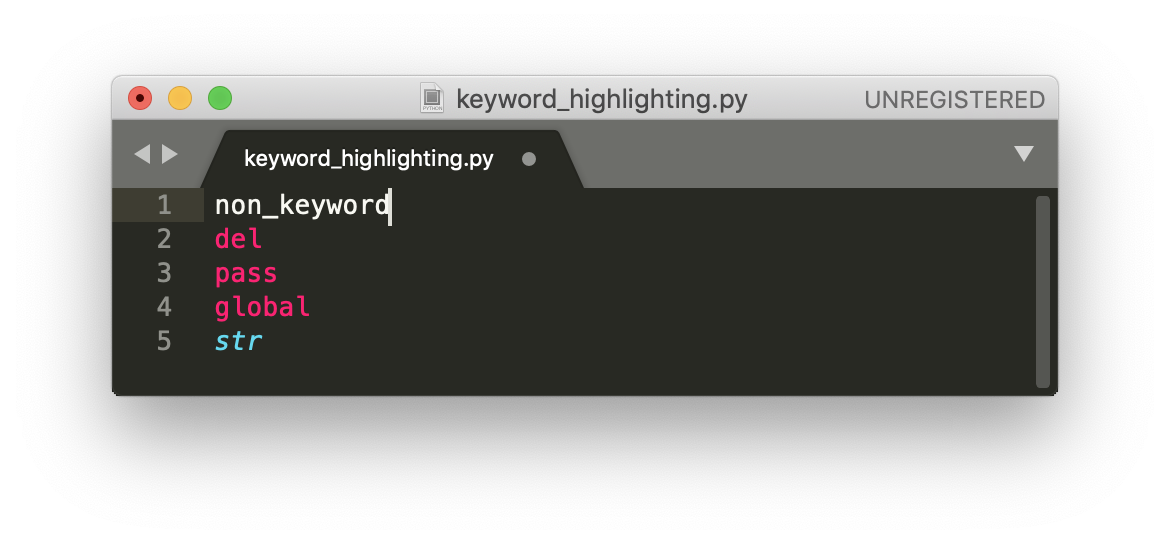
\includegraphics[width = .53\textwidth]{images/sublime_keyword_highlight.png}
\end{center}

While you simply can't assign any value to \code{class}, you can assign a value to \code{str}. Even though it's permitted, I would suggest you never assign a value to \code{str} because it can be used to confirm something is a string type. The same goes for keywords like \code{int}. Consider the program below. 

\begin{lstlisting}
s = 'Python'
is_string = type(s) == str
\end{lstlisting}

The above works so that \code{is_string} holds a value \code{True} if and only if \code{s} is a string. In this case, \code{is_string = True} The program below also runs, but it does something different. \code{str} holds the value \code{10} so the last line checks if the type of \code{s} is equal to ten. Now, \code{is_string} holds the value \code{False}.

\begin{lstlisting}
s = 'Python'
str = 10
is_string = type(s) == str
\end{lstlisting}


Finally, consider how the variables chapter in \cite{lubanovic2019introducing} opens with a quote from \link{https://www.biblegateway.com/passage/?search=Proverbs\%2022\%3A1&version=NRSV}{Proverbs 22:1}. ``A good name is rather to be chosen than great riches.'' In its Biblical context, this expresses the idea that a good reputation is better than money and that the name is an expression of the inner character of its bearer. \cite{lubanovic2019introducing} is stressing the importance of variable names in a different way. Well-named variables help the reader and user of your code. In a way, instead of indicating the character of the person, variable names actually shape the character of your code. Be thoughtful of this, so if you're using \code{n} for the number of apples, perhaps you can spare the keystrokes for \code{num_apples}. We might complete the Biblical analogy by saying that readable code with well-named variables is better than confusing code that might run faster or have been written faster. This concern for readability brings us to our next topic, comments. 


\section{Comments}
\noindent \textit{Comments are briefly addressed in \cite{lubanovic2019introducing} Chapter 4.}

Commenting your code is helpful if you care about your colleagues or your future self. Comments should add clarity to
the intention and workings of code. A comment is a piece of code that isn't actually executed---it's a comment left for the reader or the person who inherits and modifies your code.
Everything after a \lstinline[language = Python]{#} will be ignored by the Python interpreter.

\begin{lstlisting}[language = Python]
# This will print a greeting.
print('Hello, World!') \end{lstlisting}

\smallskip
 You might also use end-line comments like the following

\begin{lstlisting}[language = Python]
print('Hello, World!') # Prints a greeting \end{lstlisting}

\smallskip

 PEP 8 addresses comments \textcolor{blue}{\href{https://www.python.org/dev/peps/pep-0008/\#comments}{here}}.
I don't intend to grade based on the stylistic orthodoxy of your comments, but spaces are free so I do recommend 
\lstinline[language = Python]{# Comments like this} instead of \lstinline[language = Python]{#Comments like this}.

Perfect comment technique does not correct for bad code though. Compare the following blocks of code. 

\begin{lstlisting}
x = 90 # Wins
y = 10 # Losses
z = x/y # Win Loss Ratio
a = 100 * x/(y+x) # Winning Percentage
\end{lstlisting}

\begin{lstlisting}
wins = 90
lossses = 10
win_loss_ratio = wins/losses
winning_percentage = 100 * wins / (losses + wins)
\end{lstlisting}

The first block is commented and the second is not. Still, the second code block is much better because the variable names are chosen so you don't \emph{need} comments. Good naming becomes even more important as the program becomes longer and the variable is used over and over. See also the discussion in \cite{long2021}.



\section{Data Types and Conversion}

To start, we are concerned with strings, integers, and floats. In Python, these are classes 
\lstinline{str}, \lstinline{int}, and \lstinline{float}.
You can check the type of variable or value using \code{type()}.


\begin{lstlisting}[language = Python]
string_example = ''
int_example = -1
float_example = -1. \end{lstlisting}

\smallskip
 Some types can be converted by using \lstinline[language = Python]{str()},
\lstinline[language = Python]{int()}, or \lstinline[language = Python]{float()}. You might informally call these functions, but they actually aren't because function has a special meaning that's reserved for other things. We'll call them callables, which is a more general category. 


\begin{lstlisting}
print(type(1))
print(type(str(1)))
\end{lstlisting}

\section{Input}

It's not that common for a data science workflow, but you can read input using \lstinline[language = Python]{input()}.
The input is always read in as a string.

\begin{lstlisting}[language = Python]
favorte_color = input("What is your favorite color?")
favorite_number = input("What is your favorite number?")
attending_in_person = input("I am attending class in person.") \end{lstlisting}


\section{Calculations}

You can use Python as a calculator. Below is the list of operations and symbols. 

\begin{center}
{\setlength{\tabcolsep}{2em}
\begin{tabular}{lll}
\toprule
Operator & Description \\
\midrule
\code{+} &    Addition \\
\code{-} & Subtraction \\
\code{*}  &    Multiplication \\
\code{/}  &   Floating point (normal) division \\
\code{//}  &  Integer (truncating) division \\
\code{\%} & Modulus (remainder) \\
\code{**} & Exponentiation \\
\bottomrule
\end{tabular}}
\end{center}


What might stand out is 
\begin{itemize}
\item Exponentiation is done with \lstinline[language = Python]{**}, not \lstinline[language = Python]{^}.
\item Integer division (rounds down) is done with \lstinline[language = Python]{//}.
\item The remainder of $x$ divided by $y$ can be found with \code{x \% y}, which might be read as
$x$ \emph{modulo} $y$. 
\end{itemize}

If a float is involved in an operation, the result will also be a float, as in \code{type(2 + 2.)}.
